\vspace{-1pt}
\section{Obtaining Populations for Community Detection} 
The populations used in this study are drawn from social media with a particular focus on datasets with node attributes, such as text, and a social network structure. Moreover, we want datasets where the underlying communities come from different backgrounds. To satisfy this, we utilized two different datasets: Gamergate and U.S. Presidential Election. Both datasets have ground truth community labels. Our process for obtaining these labels will be discussed in detail.
\subsection{Gamergate}
The Gamergate dataset consists of tweets posted in 2014 between months of August through October. The tweets surround the Gamergate controversy~\cite{mortensen2018anger}. It contains 21,441 users who collectively produced 104,914 tweets. These users fall into one of the two groups surrounding the controversy. One group consists of Gamergate supporters who are tweeting about ethics in journalism and believe that regardless of the relationship between journalists and game developers, journalists should give honest reviews to game developers. %FM: Who is "them"? Could you clarify?
%NM: Fixed it!
The other group, Gamergate opposers, argues that Gamergate supporters attack female game developers and also feminist critics, and that they are not concerned with ethics in journalism, but are using the opportunity to attack women in the gaming industry.

In this study, we conducted an Amazon Mechanical Turk experiment discussed later in the paper to obtain ground truth labels for each of the users in this controversy. The retweet network of this dataset is shown in Figure \ref{Gamergatenetwork}.
\begin{figure}[H]
  \centering
  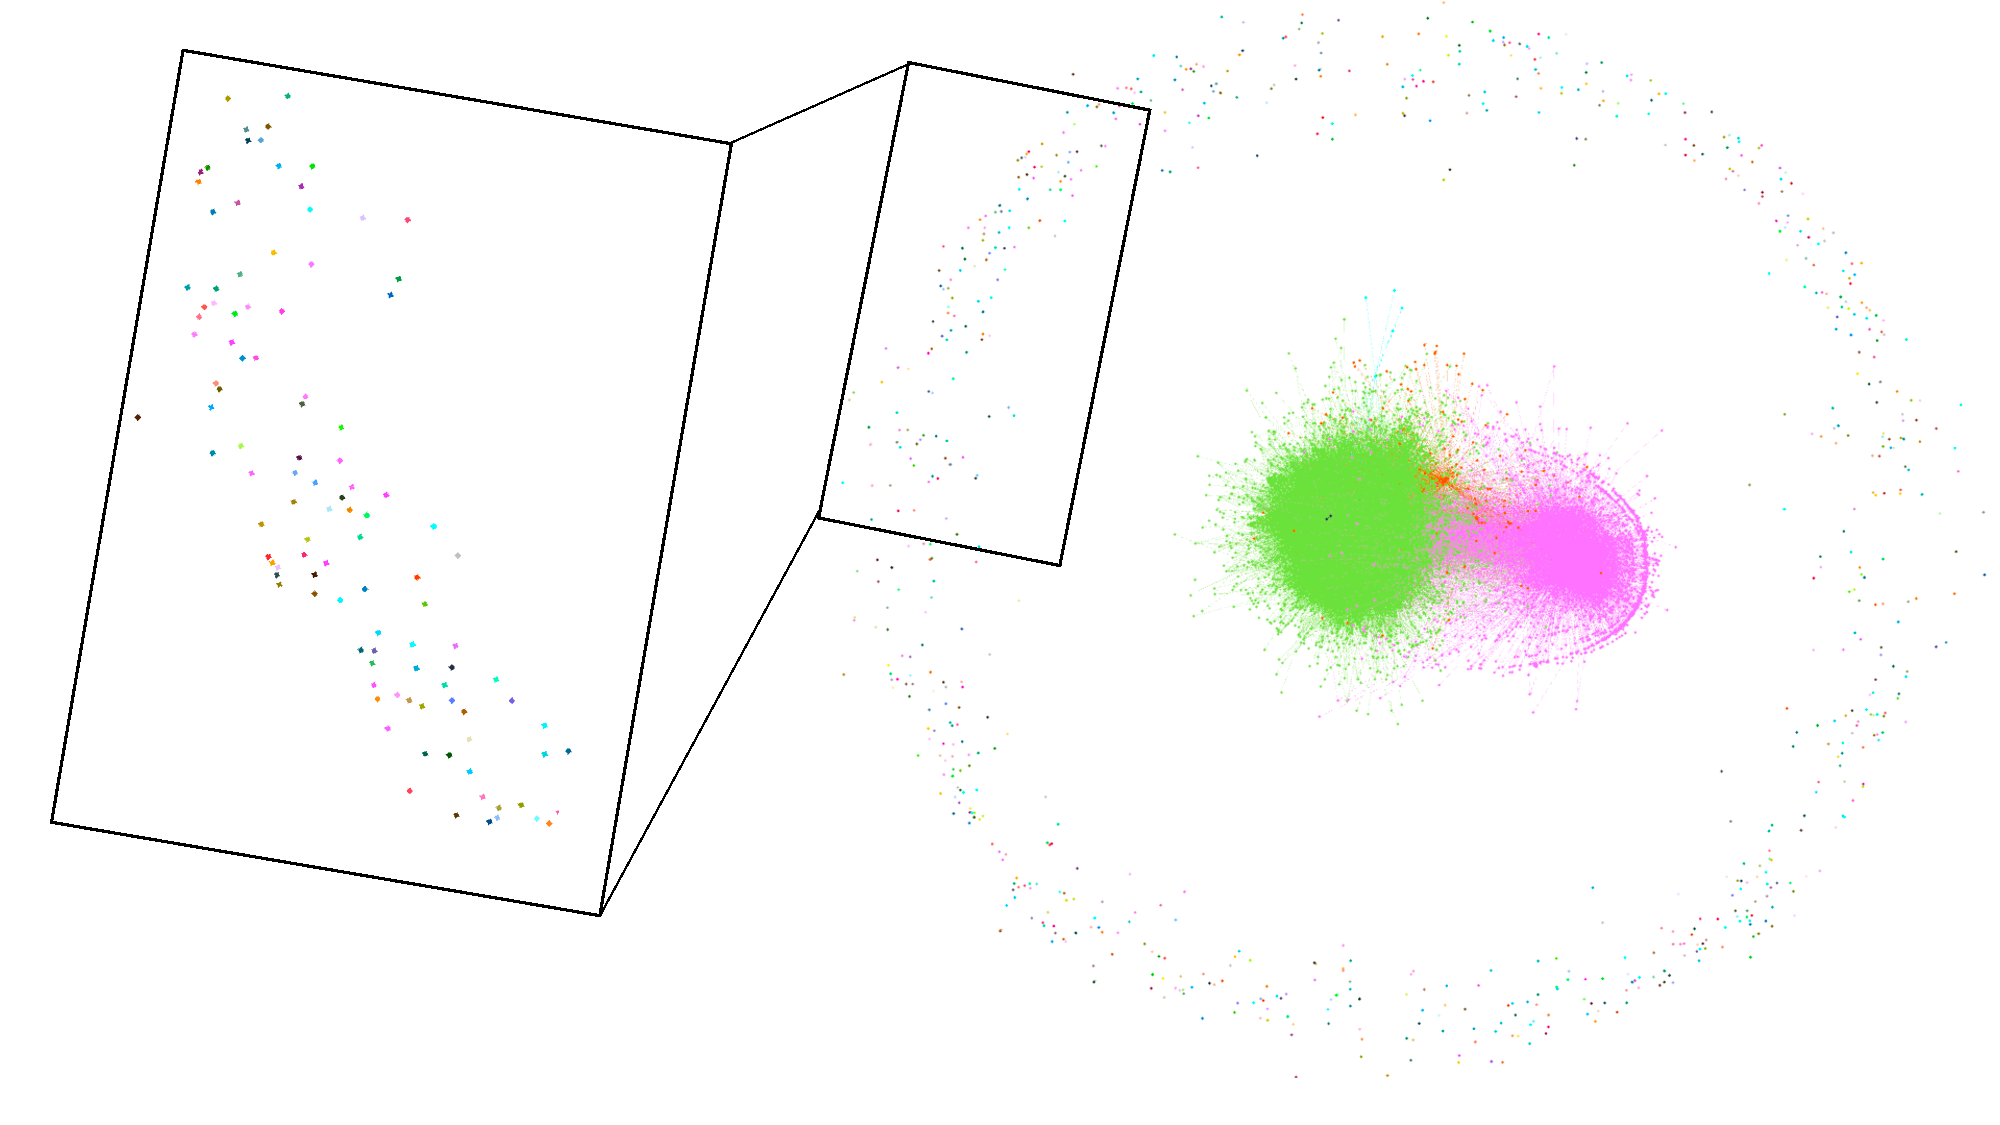
\includegraphics[width=0.5\textwidth,height=8cm]{cool_election.pdf}
  \caption{The 2016 U.S. presidential election seed-user retweet network colored by the  political party from modularity. The callout emphasizes the low-degree users.}
  \label{electionpic}
\end{figure}
\subsection{U.S. Presidential Election}
This dataset contains 10,074 users who discuss the U.S. presidential election in 2016. This dataset consists of two major groups which indicate the political party of each user. This dataset comes from~\cite{badawy2018characterizing} in which we only utilized the seed users from the whole dataset which brought our dataset size down from more than million users to 10,074 users since we required pure ground truth labels that were obtained away from the network structure and label propagation. The network structure of this dataset is shown in Figure \ref{electionpic}.  
\section{Obtaining Ground Truth Labels for Gamergate}
Unlike the 2016 presidential election dataset, the Gamergate dataset inherently lacks ground truth labels for each user. To obtain them, we conducted an Amazon Mechanical Turk experiment in which we asked human annotators to assign labels to each user in the Gamergate dataset.
\subsection{Experimental Setup}
In order to collect labels for each user in the Gamergate dataset, all the tweets associated to a user were mapped to the particular user so that the dataset was on a user level. Out of 21,441 total users, we excluded users who had only single tweets and duplicated users with same tweets. We then asked the turkers on Amazon Mechanical Turk to label each of the 8,128 users left based on their tweets into one of the following groups:
\begin{enumerate}
\item Gamergate Supporter: Users fighting for ethics in journalism and criticizing some women game-developers and journalists for their unethical relationships.
\item Gamergate Opposer:  Users advocating for women's rights and protecting attacks from Gamergate supporters to female game-developers and feminist advocates.
\item Unaffiliated: Users who belong to neither of the groups.
\end{enumerate}
Turkers were given complete description of the controversy and a detailed explanation of the labeling procedure. In order to make sure that the turkers were following the standards, some sanity check questions were put under each page for us to be able to identify bot turkers. These sanity check questions were trivial, made-up users with tweets that were easy to be categorized into one of the three groups, Gamergate Opposer, Gamergate Supporter, and Unaffiliated. After identifying bot turkers and excluding their labels from the total labels, we took the maximum agreement between 8,128 users that were labeled by at least three turkers. This resulted in a new dataset discussed in the next section which served as our ground truth.
\subsection{Dataset}
The Gamergate dataset had 21,441 users initially. In this study, we consider only users who posted at least two original tweets. The resulting dataset contains %After doing some preprocessing on this dataset by deleting the singleton users who had only one tweet % FM: How do we define singletons? We should be very careful here..  
%NM: fixe it!
8,128 users which were then labeled by the turkers. After analyzing the Turker agreement between 8,128 labeled users, we considered only users where turkers agreed two out of three times on a single label. After this filtering, we have 7,320 labeled users in total. These 7,320 users served as our ground truth labels.
\begin{figure}[H]
  \centering
  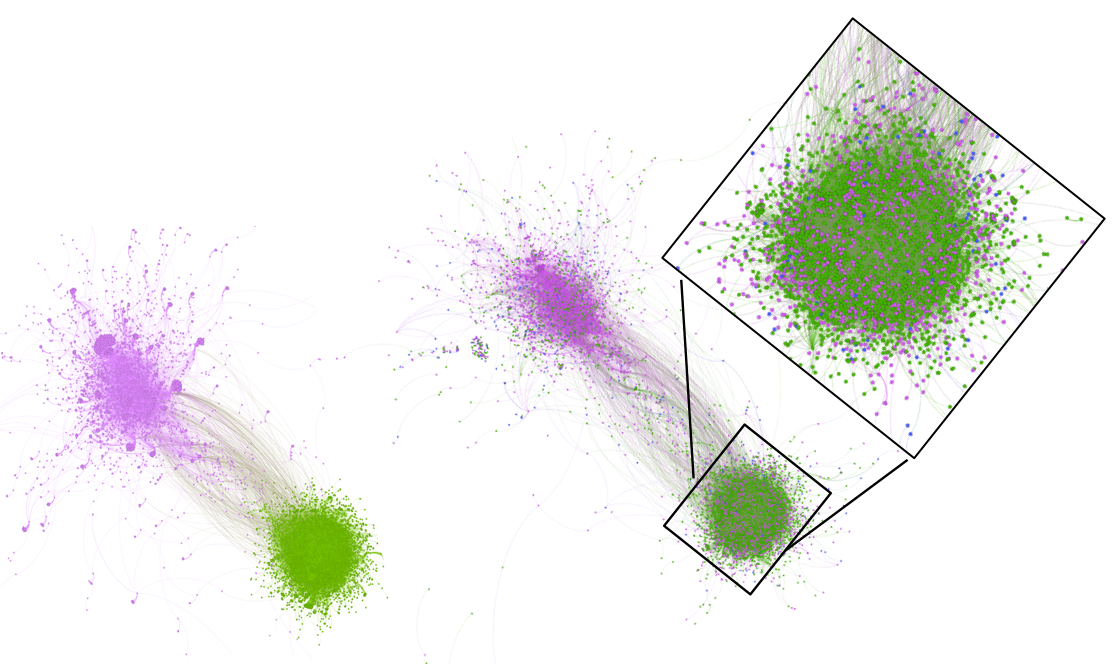
\includegraphics[width=0.46\textwidth]{mturk.png}
  \caption{The Gamergate retweet network colored based on the network structure is shown on the left hand side, and the network colored by the ground truth labels is shown on the right hand side. The callout zooms one of the components, showing the disagreement between the two labeling approaches. Purple nodes represent Gamergate opposers and green nodes represent Gamergate supporters.}
  \label{Gamergatenetwork}
\end{figure}
\subsection{Results}
After obtaining the ground truth labels and having three ground truth groups of users, Gamergate supporters, Gamergate opposers, and unaffiliated, the communities obtained using network attributes were then compared with the groups obtained by the labels from the Mechanical Turk experiment. Surprisingly these results had a very low agreement which will be discussed in detail in "Community Detection Results" section. Figure \ref{electionpic} confirms this fact by showing the disagreement between the left hand side picture, which is colored based on the network structure, and the picture on the right colored by the ground truth labels. There is a significant amount of disagreement between these two results. The purple nodes represent Gamergate opposers and the green nodes represent Gamergate supporters. Using network structure and attributes would put almost all of Gamergate supporters in the green portion of the network and Gamergate opposers in the purple section of the network completely separated; however, the ground truth labels tend to have mixed users into each of the sections. The ground truth results are expected as many opposers may retweet Gamergate supporters; therefore, using network attributes merely on the retweet network might not be a good idea for separating these users, and other attributes and characteristics of users can be used for a more accurate community detection task. These results illustrate the fact that network does not explain everything and additional information is required in order to obtain accurate communities of users. This motivated us to come up with a new method that would not only address the bias from creating small communities and exclusion of low-degree nodes but would also have higher agreement with the ground truth communities by using other node attributes in addition to the network structure which will be discussed in the next section.
